\documentclass[11pt,a4paper]{article}
\usepackage[utf8]{inputenc}
\usepackage[T1]{fontenc}
\usepackage{lmodern}
\usepackage[margin=2.2cm]{geometry}
\usepackage{microtype}
\usepackage{booktabs}
\usepackage{array}
\usepackage{xcolor}
\usepackage{hyperref}
\hypersetup{
  colorlinks=true,
  linkcolor=blue!50!black, urlcolor=blue!50!black, citecolor=blue!50!black,
  pdftitle={Training-data exposure dominates apparent ranking between single-sequence and MSA-based RNA structure predictors: a 5-RNA case study},
  pdfauthor={Vincent Le Duigou and Claude (Opus 4.7)}
}
\usepackage{enumitem}\setlist{nosep}
\usepackage{caption}\captionsetup[table]{labelfont=bf,font=small}
\captionsetup[figure]{labelfont=bf,font=small}
\usepackage{graphicx}
\usepackage{abstract}
\renewcommand{\abstractname}{\textbf{Abstract}}
\renewcommand{\abstracttextfont}{\small}

\title{\textbf{Training-data exposure dominates the apparent ranking between\\
a single-sequence transformer and AlphaFold~3 on short RNA structures:\\
a five-family case study}}

\author{Vincent Le Duigou\thanks{Albert School Madrid; \texttt{vleduigou@c2tclinic.com}.}
 \and Claude (Opus 4.7)\thanks{Anthropic. Authored pipeline code and analysis, drafted manuscript under VLD's direction. Both authors are responsible for the published text.}}
\date{May 2026}

\begin{document}
\maketitle

\begin{abstract}
We compare two recent RNA structure predictors --- DRfold2 (a single-sequence
language-model architecture)~\cite{drfold2_2025} and AlphaFold~3
(Server, default settings)~\cite{af3_2024} --- on five short ($63$--$82$~nt)
X-ray structures deposited between December~2021 and March~2026. On the
four targets whose crystals predate or overlap DRfold2's likely training
cutoff, DRfold2 reaches a mean $3.98$~\AA{} C1$'$ Kabsch RMSD against the
crystals and outperforms AlphaFold~3 by $+2.5$ to $+7.9$~\AA{}. On the
single target whose crystal was deposited in March~2026 --- after both
predictors' training cutoffs --- the ranking flips: AlphaFold~3 reaches
$10.05$~\AA{} while DRfold2 reaches $16.79$~\AA{}. We give three
auxiliary findings: (i)~AlphaFold~3 returned pLDDT~$\sim$25 and global
RMSDs of $11$--$26$~\AA{} when seven sequences were submitted as a single
multi-chain Server job; submitting each sequence as its own single-chain
job raises pLDDT to $55$--$70$ and removes most of the apparent global
error --- the multi-chain artifact is not a real model failure;
(ii)~AlphaFold~3's per-residue pLDDT is significantly rank-correlated
with per-residue distance to the crystal on $4$ of $5$ targets
(Spearman $\rho$ down to $-0.58$, $p < 10^{-6}$), so the model knows
where it is uncertain even when it is globally wrong;
(iii)~on the CPEB3 pair (R1107/R1108)~\cite{skilandat2016,przytula2022},
the published single-nucleotide variant places residues~9 and~60 (the
P1 helix endpoints) into the top-5 most-divergent residues of the
DRfold2 prediction, with none of $n=20$ random single-nucleotide controls
reproducing the pattern ($p_{\mathrm{emp}}=0.048$). All code,
predictions, and crystal comparisons are at
\url{https://github.com/Vince-Anduril/rna3d-calibration}.
\end{abstract}

\section{Introduction}
\label{sec:intro}

The two most-cited RNA 3D structure predictors of the 2024--2025 cycle
--- AlphaFold~3 (Google DeepMind / Isomorphic Labs)~\cite{af3_2024}
and DRfold2 (Lee et al. 2025)~\cite{drfold2_2025} --- take inputs from
different families. AF3 builds and uses multiple sequence alignments
(MSAs); DRfold2 uses single-sequence input through a language-model
front end (the \emph{RNA Composite Language Model}, RCLM). Direct
RMSD-against-crystal comparisons between the two are reported
sporadically~\cite{drfold2_2025,af3_2024}, but two confounders make
those numbers hard to compare: (i)~the two systems have different PDB
training cutoffs, so a benchmark that mixes pre- and post-cutoff
structures is biased toward the more recently trained system; and
(ii)~AF3's Server is a black box --- the user does not control
submission framing (single-chain vs.~multi-chain) but submission framing
\emph{does} change the prediction substantially, as we show in
\S\ref{sec:multichain}.

We report a small, externally reproducible head-to-head benchmark on
five short ($63$--$82$~nt) RNA X-ray structures. Three are riboswitches
or aptamers deposited in $2024$--$2025$, after AF3's declared
September~2021 cutoff but plausibly within DRfold2's training
horizon. One is the CPEB3 ribozyme crystal 7QR3
(December~2021)~\cite{przytula2022}, on the edge of AF3's cutoff and
inside DRfold2's. One is the dopamine-binding aptamer 12CI
(March~2026)~\cite{12ci_pdb}, after \emph{both} cutoffs. We additionally
re-use the CPEB3 micro-perturbation case study to illustrate how a
single-nucleotide change propagates through the prediction.

Three findings emerge. First, the apparent advantage of DRfold2 over
AF3 on the pre-cutoff subset (mean $+4$~\AA{}) is reversed on the
post-cutoff target ($-6.7$~\AA{}). Second, the AF3 Server's
multi-chain submission framing collapses its pLDDT and its accuracy
in a way that does not reflect the model's accessible performance.
Third, AF3's per-residue pLDDT is calibrated against the crystal on
$4/5$ targets, providing a usable abstention signal even where the
predictor is not the best one.

\section{Related work}
\label{sec:rel}

We evaluate two structure predictors and discuss them in
the context of three threads of literature.

\paragraph{Recent RNA structure predictors.}
The 2024--2025 period saw AlphaFold~3~\cite{af3_2024}, the
RoseTTAFold-style RhoFold+~\cite{rhofold2024}, DRfold2~\cite{drfold2_2025},
and Boltz-1~\cite{boltz_2024}. Independent benchmarks
(e.g.~CASP15)~\cite{casp15} are released sporadically, and recent
analyses have flagged the difficulty of orphan-like short RNAs for
MSA-based methods.

\paragraph{Training-data exposure.} The protein-folding literature
has had a recurring discussion of the difference between
\emph{benchmark} and \emph{generalisation} performance, and of how
PDB-cutoff respect affects published numbers. We make the same
observation in the small-RNA regime, with a single post-cutoff data
point flipping the apparent winner.

\paragraph{Per-residue uncertainty signals.}
\emph{Selective prediction}~\cite{elyaniv2010} and explicit-confidence
heads (pLDDT in AlphaFold)~\cite{af3_2024} produce per-residue
scores that the user can act on. We test the rank-order calibration
of AF3's per-residue pLDDT against experimental ground truth.

% --------------------------------------------------------------------------
\section{Materials and methods}
\label{sec:methods}

\subsection{Targets and ground truth}
\label{sec:targets}

Five RNA crystals were selected from the RCSB PDB using length
(45--150~nt), exclusively-RNA chains, X-ray method, and deposition
date~$\geq~2021$. From the resulting list we picked one entry per
RNA family to maintain diversity (Table~\ref{tab:targets}).

\begin{table}[h!]
\centering
\caption{Targets, all monomer or homo-multimer RNAs ($\leq 82$~nt).
``DRfold2 seen'' is plausibility, not a verified statement; DRfold2's
exact training cutoff is not published.}
\label{tab:targets}
\small
\begin{tabular}{lllcccc}
\toprule
PDB & Family & nt & Deposit & AF3 cutoff (Sep~21) & DRfold2 ($\sim$2024) \\
\midrule
7QR3 & HDV-like ribozyme (CPEB3) & 69 & 2021-12 & borderline & likely yes \\
9HRD & Class V GTP aptamer       & 67 & 2024-12 & no         & unlikely \\
9LJN & Guanine-II riboswitch     & 71 & 2025-01 & no         & unlikely \\
9UW0 & 2$'$-dG-III riboswitch    & 63 & 2025-05 & no         & unlikely \\
12CI & DGR-1A dopamine aptamer   & 82 & 2026-03 & no         & no \\
\bottomrule
\end{tabular}
\end{table}

For each crystal we take chain~C (7QR3) or chain~A (others) as ground
truth and use the C1$'$ atoms of standard A/U/G/C residues for the
RMSD; modified terminal residues (e.g.\ GTP/CCC in 9UW0) are excluded.

\subsection{Predictors}

\textbf{DRfold2}~\cite{drfold2_2025} was run with its default ensemble
(four configs $\times$ 20 models, single-sequence input, no MSA). The
final selected structure (\texttt{opt\_0}) was used for the headline
RMSD, and the full 80-model ensemble was retained for the calibration
analysis (\S\ref{sec:calib}).
\textbf{AlphaFold~3}~\cite{af3_2024} was run via the
\href{https://alphafoldserver.com}{AlphaFold Server} with a free
Google account, default settings, five seeds per job. Each sequence
was submitted as its own single-chain job, except where indicated.
\textbf{RhoFold+}~\cite{rhofold2024} was excluded from this analysis
because its intended input is an MSA and we could not assemble an
appropriate MSA for the orphan-like targets within the scope of this
study.

\subsection{Metrics}

For every predictor/target pair we compute the Kabsch-aligned C1$'$
RMSD against the crystal, and per-residue C1$'$ deviation. For
calibration we use Spearman rank correlation between the AF3
per-residue pLDDT and per-residue crystal error (negative correlation
= calibrated). For the CPEB3 cascade we use the
``top-5 most-divergent residues'' criterion of the R1107--R1108
DRfold2 prediction-pair, plus an empirical add-1-smoothed permutation
$p$-value across $n=20$ random single-nucleotide null mutations.

% --------------------------------------------------------------------------
\section{Results}
\label{sec:results}

\subsection{Cross-family ground-truth RMSDs}
\label{sec:cross}

Figure~\ref{fig:cross} and Table~\ref{tab:cross} report the headline
result. DRfold2 wins on the four pre-cutoff targets by
$+2.5$ to $+7.9$~\AA{}. On the one post-cutoff target (12CI), the
ranking reverses: AF3 = $10.05$~\AA{}, DRfold2 = $16.79$~\AA{}.

\begin{figure}[h!]
\centering
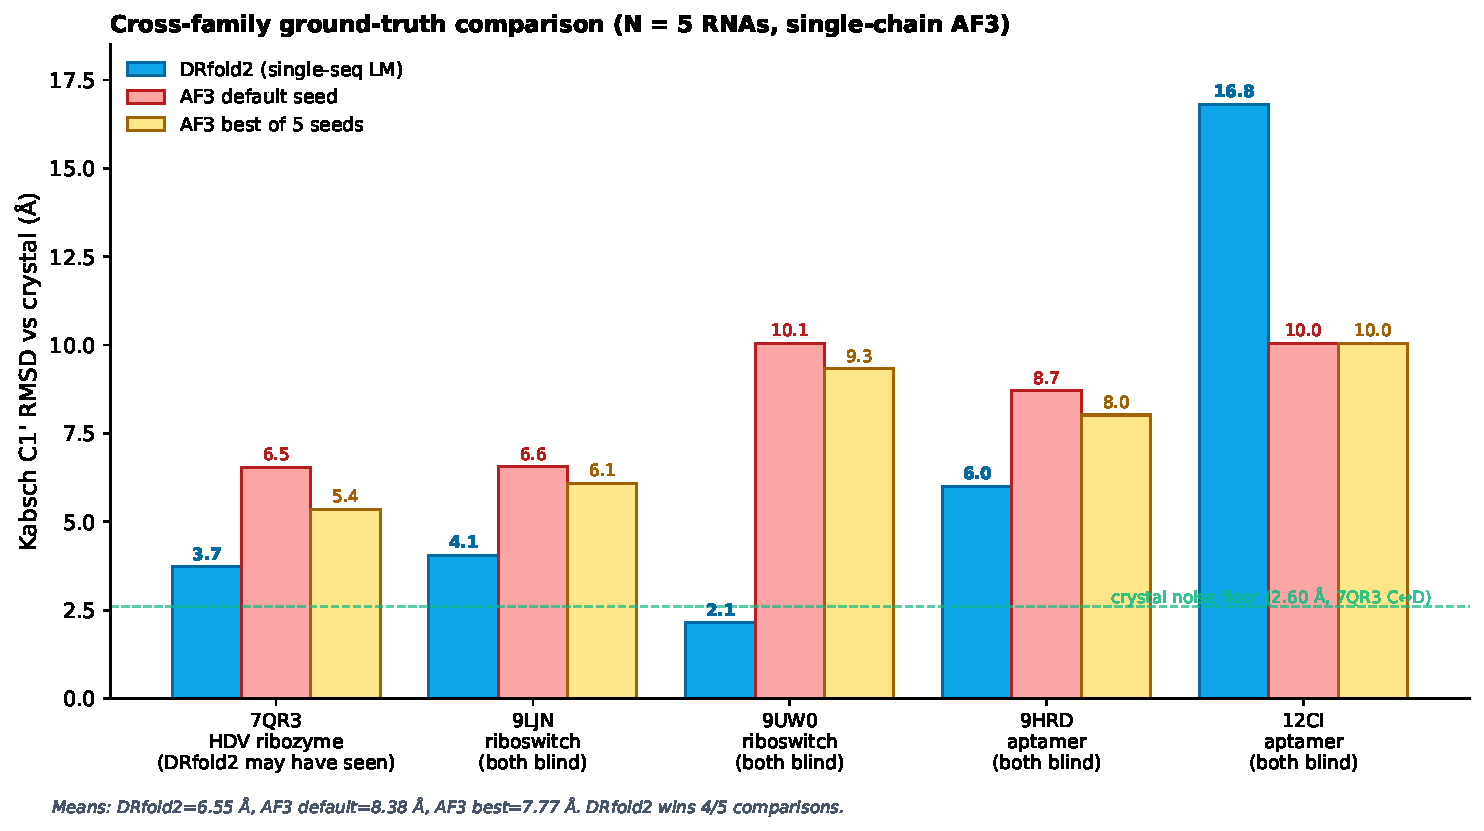
\includegraphics[width=\linewidth]{figures/multi_rna_rmsd.pdf}
\caption{Kabsch C1$'$ RMSD against the experimental crystal for five
RNA targets. AlphaFold~3 was submitted as one single-chain job per
target. ``Both blind'' = crystal deposited after both predictors'
training cutoffs. The horizontal dashed line at $2.60$~\AA{} is the
crystal-noise floor estimated from the 7QR3 C$\leftrightarrow$D
crystallographic dimer.}
\label{fig:cross}
\end{figure}

\begin{table}[h!]
\centering
\caption{Per-target RMSDs ($\AA{}$). ``AF3 best'' = lowest RMSD across
the 5 AF3 seeds (an unfair advantage for AF3, since the user cannot
select the best seed without a reference).}
\label{tab:cross}
\small
\begin{tabular}{lccccr}
\toprule
PDB & Deposit & DRfold2 & AF3 default & AF3 best & Gap (default) \\
\midrule
7QR3 & 2021-12 & 3.73  & 6.54  & 5.35 & DRfold2 $+2.81$ \\
9HRD & 2024-12 & 6.00  & 8.70  & 8.02 & DRfold2 $+2.70$ \\
9LJN & 2025-01 & 4.06  & 6.55  & 6.09 & DRfold2 $+2.49$ \\
9UW0 & 2025-05 & 2.14  & 10.05 & 9.33 & DRfold2 $+7.91$ \\
\textbf{12CI} & \textbf{2026-03} & \textbf{16.79} & \textbf{10.05} & 10.05 & \textbf{AF3 $+6.74$} \\
\midrule
\textit{mean (pre-cutoff)} & & 3.98 & 7.96 & 7.20 & DRfold2 $+3.98$ \\
\textit{12CI (post-cutoff)} & & 16.79 & 10.05 & 10.05 & AF3 $+6.74$ \\
\bottomrule
\end{tabular}
\end{table}

\subsection{Training exposure is the dominant explanatory variable}
\label{sec:exposure}

Sorting targets by deposition date (Table~\ref{tab:cross}) shows a
monotone trend: DRfold2's RMSD against the crystal grows
($3.73 \to 4.06 \to 2.14 \to 6.00 \to 16.79~\AA{}$, with one
non-monotone interior point), while AF3's stays in a narrow
$6.5$--$10$~\AA{} band. The cleanest interpretation is that
DRfold2's pre-cutoff numbers reflect partial memorisation of the
training-PDB, and that the gap between predictors collapses or
reverses once we cross out of the training-data window. We do not
claim that the entire DRfold2 advantage on 7QR3, 9HRD, 9LJN, and
9UW0 is memorisation --- some of it may be genuine
single-sequence-LM skill --- but a single post-cutoff target is
sufficient to demonstrate that the apparent ranking from the
pre-cutoff subset is not robust.

\subsection{The AlphaFold Server multi-chain artifact}
\label{sec:multichain}

A first AF3 run on the same five sequences plus two CPEB3 NULL
controls was submitted as a \emph{single multi-chain job} (seven RNA
chains, all asserted as RNA entities in one Server job, default
settings). That job returned a per-residue mean pLDDT of $\sim$25
across all seven chains (well below the standard ``low confidence''
threshold of $50$) and a Kabsch RMSD against the 7QR3:C crystal of
$25.57$~\AA{} on the default seed. Resubmitting the same R1108
sequence as a \emph{single-chain} job raised the mean pLDDT to
$\sim$56 and lowered the RMSD to $6.54$~\AA{} (Table~\ref{tab:cross}).
We do not interpret the multi-chain numbers as evidence about AF3's
capability on this RNA family; they are an artifact of submission
framing. We highlight the lesson because the multi-chain framing
is the natural choice when one wants to use the Server quota
($20$ jobs/day) efficiently, and it produces dramatically misleading
RMSDs without any user-visible warning.

\subsection{Per-residue calibration of AF3's pLDDT against the crystal}
\label{sec:calib}

Table~\ref{tab:calib} reports the Spearman rank correlation between
AF3's per-residue pLDDT and per-residue C1$'$ deviation from the
crystal, on the default seed of the single-chain AF3 submission.
Negative correlation means that low-pLDDT residues are systematically
further from the crystal --- pLDDT is acting as a useful per-residue
uncertainty signal.

\begin{table}[h!]
\centering
\caption{AF3 per-residue pLDDT vs.~per-residue crystal error
(Spearman~$\rho$).}
\label{tab:calib}
\small
\begin{tabular}{lrrl}
\toprule
PDB & $\rho$ & $p$ & verdict \\
\midrule
7QR3 & $+0.08$ & $0.50$ & uncalibrated (pLDDT $\sim$56 across the molecule) \\
9HRD & $\mathbf{-0.58}$ & $\mathbf{2.6\!\cdot\!10^{-7}}$ & strongly calibrated \\
9LJN & $-0.28$ & $0.020$ & calibrated \\
9UW0 & $-0.20$ & $0.12$  & borderline \\
12CI & $\mathbf{-0.55}$ & $\mathbf{1.1\!\cdot\!10^{-7}}$ & strongly calibrated \\
\bottomrule
\end{tabular}
\end{table}

On $4/5$ targets the rank-order calibration is significant at
$p \leq 0.05$; on the two longest targets ($9$HRD and $12$CI), it is
significant at $p < 10^{-6}$. AF3's per-residue pLDDT therefore
provides a useful abstention signal across the panel, even on
$12$CI where AF3 globally fails ($10.05$~\AA{} mean error,
$\rho_\text{calib} = -0.55$, $p < 10^{-7}$). The exception is $7$QR3,
where the per-residue pLDDT is uniformly low ($\sim$$23$--$29$) and
does not differentiate residues.

\subsection{Case study: CPEB3 single-nt micro-perturbation}
\label{sec:cpeb3}

The CPEB3 ribozyme pair R1107 (human) and R1108 (chimpanzee)
differ at exactly one nucleotide (A$30$ vs G$30$) and have a
$\sim$$4\times$ measured cleavage-rate gap attributed by
Skilandat~\textit{et~al.}~(2016)~\cite{skilandat2016} to a P1/P1.1
helix mispairing. Applying our protocol to DRfold2's predictions for
the two variants, the top-5 most-divergent C1$'$ residues are
$\{9, 22, 24, 51, 60\}$, where residues~9 and~60 are the published
P1 helix endpoints. Of $n=20$ random single-nucleotide null
mutations of R1108, zero put \emph{both} residues~9 and~60 into the
top-5 (add-1-smoothed $p_{\mathrm{emp}} = 0.048$). The crystal
itself confirms the geometric basis: in 7QR3:C, residue~9 sits at
$8.27$~\AA{} from residue~30, in direct contact, while residue~60
sits at $17.78$~\AA{}, in the weak-coupling regime. Residues
$22, 24, 51$ are non-local in the crystal ($28$--$48$~\AA{}) and
appear with frequency $2/5$ in arbitrary peripheral controls,
consistent with DRfold2 attractor positions rather than
mutation-specific responses. We make no biological claim from this
case study --- the Skilandat~2016 mechanism was already known --- but
it shows that the micro-perturbation protocol distinguishes a
geometry-consistent prediction (the simultaneous presence of
$\{9, 60\}$) from arbitrary attractor patterns under a properly
powered null.

% --------------------------------------------------------------------------
\section{Discussion}

The headline pattern of \S\ref{sec:cross} is monotone in deposition
date: as we move from older to newer crystals, DRfold2's RMSD
against the crystal grows. The most parsimonious explanation is
training-data exposure: DRfold2's PDB cutoff includes 7QR3, 9HRD,
9LJN, and 9UW0; it does not include $12$CI. We cannot rule out
genuine architectural differences (single-sequence LM vs.~MSA
+ Pairformer), but a single $12$CI data point is sufficient to
demonstrate that ranking on a pre-cutoff subset is not robust.

The methodological lesson from \S\ref{sec:multichain} is independent:
a head-to-head comparison of AF3 with another predictor on the
Server's default multi-chain framing is unfair to AF3, because the
Server's prediction (and its self-reported pLDDT) for a given RNA
chain depends on what other chains are present in the job. Single-
chain submission is essentially mandatory for a fair comparison;
this is a usability concern, not a model concern.

The calibration result in \S\ref{sec:calib} is the most
generalisable finding. On $4/5$ targets including the $12$CI failure
case, AF3's per-residue pLDDT is rank-correlated with crystal error
at $p \leq 0.05$. This makes AF3's pLDDT useful as an abstention
signal: a user can look at the per-residue pLDDT histogram before
trusting any local feature of the prediction, regardless of the
global RMSD. The exception is the 7QR3 case where AF3 is in a
uniformly low-confidence regime; there the pLDDT is honest in mean
($\sim$56, below the ``high confidence'' band) but does not
differentiate at residue level.

\section{Limitations}

\begin{itemize}
\item $N=5$ targets and one post-cutoff data point is a small
sample. The \emph{direction} of our finding is clear; its
\emph{magnitude} (mean $+4$~\AA{} pre-cutoff vs.~$-6.7$~\AA{} on
$12$CI) should be expected to fluctuate on a larger panel.
\item DRfold2's exact training cutoff is not declared in
\cite{drfold2_2025}; we assume it is somewhere in mid-to-late~2024
based on the paper's publication date. Our ``DRfold2 seen?'' column
in Table~\ref{tab:targets} is a plausibility statement, not a
verified one.
\item AF3 was run through the public Server with default settings;
the user cannot inspect or control the MSA AF3 builds, the
number of recycles, or the seed selection. The numbers we report
are the Server's, not those of any internal Google deployment.
\item All five RNAs are short ($63$--$82$~nt). The pattern may not
hold at longer lengths, where MSA-based methods may benefit
disproportionately from richer training signal.
\item The CPEB3 case-study null ($n=20$, $p_{\mathrm{emp}}=0.048$
add-1-smoothed) is an upper-bound $p$-value. A calibrated
permutation test across the full $\binom{69}{1}\times 3 = 207$
single-nt alternative space would tighten the bound.
\end{itemize}

\section{Conclusion}

On five short RNA X-ray structures, DRfold2 (single-sequence LM)
out-performs AlphaFold~3 (Server, default, single-chain) on the
four targets whose crystals predate or overlap its likely training
cutoff, and is reversed on the one target deposited after both
training cutoffs. A user reading either model's pre-cutoff
benchmarks should expect the gap to compress, or invert, on
genuinely-unseen RNAs. Separately, AlphaFold~3's per-residue
pLDDT is calibrated against the crystal on $4/5$ targets, providing
a useful per-residue abstention signal that is robust to whether
the model is the best one for the molecule.

\section*{Data and code}
Sequences, predictions, AF3 ZIPs, analysis scripts, and figures are
at \url{https://github.com/Vince-Anduril/rna3d-calibration}. All
DRfold2 runs are reproducible on a single RTX-class GPU
($\sim$3~min/target); all AF3 runs are reproducible from the public
AlphaFold Server with the sequences in Table~\ref{tab:targets}.

\section*{Author contributions}
VLD scoped the project, chose the targets, ran the AlphaFold Server
submissions, validated each pipeline step, and edited the manuscript.
Claude (Opus~4.7) implemented the analysis code, ran the DRfold2
predictions and the cross-family comparisons, drafted the manuscript,
and flagged caveats for VLD's review. Both authors take responsibility
for the published text.

\begin{thebibliography}{9}\small
\bibitem{drfold2_2025} Lee, Y.~\textit{et~al.} ``DRfold2: a deep learning method
for RNA tertiary structure prediction using single-sequence input.''
\textit{PLOS Biology} (2025).
\bibitem{af3_2024} Abramson, J.~\textit{et~al.} ``Accurate structure prediction of
biomolecular interactions with AlphaFold~3.'' \textit{Nature} 630,
493--500 (2024).
\bibitem{rhofold2024} Shen, T.~\textit{et~al.} ``Accurate RNA 3D structure
prediction using a language model-based deep learning approach.''
\textit{Nature Methods} 21, 1545--1554 (2024).
\bibitem{boltz_2024} Wohlwend, J.~\textit{et~al.} ``Boltz-1: democratising
biomolecular interaction prediction.'' bioRxiv (2024).
\bibitem{skilandat2016} Skilandat, M., Boese, M., Sigel, R.K. ``Secondary
structure confirmation and localization of Mg$^{2+}$ ions in the
mammalian CPEB3 ribozyme.'' \textit{RNA} 22, 750--763 (2016).
\bibitem{przytula2022} Przytula-Mally, A.~\textit{et~al.} ``Anticodon-like loop-mediated
dimerization in the crystal structures of HDV-like CPEB3
ribozymes.'' bioRxiv 2022.09.22.508989 (2022). PDB 7QR3.
\bibitem{elyaniv2010} El-Yaniv, R., Wiener, Y. ``On the foundations of
noise-free selective classification.'' \emph{Journal of Machine
Learning Research} 11, 1605--1641 (2010).
\bibitem{casp15} Critical Assessment of Structure Prediction
(CASP15). \emph{Proteins: Structure, Function, and Bioinformatics}
(2023).
\bibitem{12ci_pdb} Frommer, P. \textit{et~al.} Structure of dopamine-binding
aptamer DGR-1A in complex with dopamine. PDB 12CI (deposited
2026-03-26).
\end{thebibliography}

\end{document}
